\documentclass[smaller]{beamer}
\usetheme[english]{Berlin}
\usepackage{ngerman}
\useoutertheme{infolines}
\beamertemplatenavigationsymbolsempty
\setbeamertemplate{caption}[numbered]
\usepackage{pgfplots,tikz,subfigure}
\usepackage{amsmath,amsthm}
\usepackage{hyperref,graphics,graphicx,color,algorithm,algorithmic,enumerate}
\usepackage{mymacros,wrapfig,relsize}
\usepackage{pict2e}
\usepackage[utf8x]{inputenc}
\usepackage{csquotes}

\newcommand{\ri}{\mathrm{i}}
\newcommand{\T}{\mathsf{T}}
\renewcommand{\H}{\mathsf{H}}
\newcommand{\eps}{\varepsilon}
\newcommand{\To}{\rightarrow}
\newcommand{\sddots}{\scalebox{0.6}{$\ddots$}}
\usepackage[pdf]{pstricks}
\usepackage{sansmathfonts}
\usepackage{eurosym}
\usepackage{ulem}
%\usepackage{arev}
%\renewcommand\familydefault{\sfdefault}

\DeclareMathOperator{\loc}{loc}
\DeclareMathOperator{\rank}{rank}
\DeclareMathOperator{\RE}{Re}
\DeclareMathOperator{\IM}{Im}
\DeclareMathOperator{\In}{In}
\DeclareMathOperator{\im}{im}
\DeclareMathOperator{\Gl}{Gl}
\DeclareMathOperator{\spa}{span}
\DeclareMathOperator{\ext}{{ext}}
\DeclareMathOperator{\ind}{ind}
\DeclareMathOperator{\normalrank}{normalrank}
\DeclareMathOperator{\essup}{ess\,sup}
\DeclareMathOperator{\vect}{vec}

\newcommand{\re}{\mathrm{e}}
\newcommand{\ddt}{\tfrac{\mathrm{d}}{\mathrm{d}t}}
\newcommand{\sys}[4]{\left[\begin{array}{c|c} #1 & #2 \\ \hline #3 & #4 \end{array}\right]}

\renewcommand{\tilde}{\widetilde}
\renewcommand{\hat}{\widehat}


\title[]{Optimierung f\"ur Studierende der Informatik}
\subtitle{-- 10. Vorlesung --}
\author[Matthias Voigt]{\textbf{Matthias Voigt$^{1,2}$}}
\institute[]{
\begin{columns}
%\begin{center}
\column{0.45\textwidth}{\centering {$^1$Universit\"at Hamburg \\ Fachbereich Mathematik \\ Hamburg \\ }}
\column{0.45\textwidth}{\centering {$^2$Technische Universit\"at Berlin \\ Institut f\"ur Mathematik \\ Berlin  \\}}
%\end{center}
\end{columns}
}
\date[]{Universit\"at Hamburg
\begin{columns}
\column{0.45\textwidth}{\centering \includegraphics[width = 1.2\textwidth]{uhh-logo.png}\\}
\end{columns}
}

\definecolor{tucgreen}{rgb}{0.0,0.5,0.27}
\definecolor{tucred}{rgb}{0.75,0,0}
\definecolor{tucorange}{rgb}{1.0,.5625,0}
\definecolor{mpired}{HTML}{990000}
\definecolor{mpigreen}{HTML}{5C871D}
\definecolor{mpiblue}{HTML}{006AA9}
\definecolor{mpibg1}{HTML}{5D8B8A}
\definecolor{mpibg2}{HTML}{BFDFDE}
\definecolor{mpibg3}{HTML}{A7C1C0}
\definecolor{mpibg4}{HTML}{7DA9A8}
\definecolor{mpigrey}{rgb}{0.9294,0.9294,0.8784}

\begin{document}

\maketitle

\begin{frame}
\frametitle{Residualgraphen}
In diesem Abschnitt wird der Begriff des \structure{Residualgraphen} vorgestellt -- ein Begriff, der besonders nützlich ist, wenn es um etwas komplexere Netzwerk-Fluss-Algorithmen geht. Statt {\glqq}Residualgraph{\grqq} sagt man auch \structure{Restgraph}. \\ \vspace*{0.2cm}

Mit $G=(V,E)$ bezeichnen wir wie bislang einen schlingenlosen Digraphen; zur Definition des Begriffs {\glqq}schlingenloser Digraph{\grqq} siehe Vorlesung 6. \\ \vspace*{0.2cm}

\textbf{Man beachte:} Aufgrund dieser Definition sind in $G$ nicht nur Schlingen ausgeschlossen, sondern auch parallele Kanten; \alert{antiparallele Kanten} (wie in der nachfolgenden Zeichnung) sind hingegen zugelassen.

\begin{center}
	\includegraphics{fig17.pdf}
\end{center}
\end{frame}

\begin{frame}
 \frametitle{Rückwärtskante von $e$}
 Bevor wir uns dem Begriff des Residualgraphen widmen, definieren wir zunächst einen zu $G$ gehörigen Graphen $G^+$, der aus $G$ dadurch entsteht, dass man zu jeder Kante $e$ von $G$ eine neue Kante hinzunimmt, die man \structure{Rückwärtskante} von $e$ nennt und mit $e^{\text{rev}}$ bezeichnet. \\ \vspace*{0.2cm}

Hier ist die genaue Definition:
\end{frame}

\begin{frame}
 \frametitle{Definition von $G^+$}
 \textbf{Definition:} Gegeben sei ein schlingenloser Digraph $G=(V,E)$ mit $m$ Kanten. Zu $G$ definieren wir $G^+$ wie folgt:
	\begin{enumerate}[i)]
		\item Die Knotenmenge von $G^+$ sei gleich $V$, d.h., $G$ und $G^+$ besitzen dieselbe Knotenmenge.
		
		\item $G^+$ enthält sämtliche Kanten von $G$.
		
		\item \alert{Darüber hinaus gebe es in $G^+$ noch $m$ weitere Kanten}: Zu jeder Kante $e=(x,y)$ von $G$ enthalte $G^+$ eine neue Kante, die wir mit $e^{\text{rev}}$ bezeichnen. Dabei gelte:
		\begin{itemize}
			\item Ist die Kante $(y,x)$ nicht in $G$ vorhanden, so sei $e^{\text{rev}} = (y,x)$.
			
			\item Ist die Kante $(y,x)$ bereits in $G$ vorhanden, so sei $e^{\text{rev}}$ eine zusätzliche Kante, die ebenfalls von $y$ nach $x$ führt. 
		\end{itemize}
	\end{enumerate}		
\end{frame}

\begin{frame}
 \frametitle{Ein Beispiel}
 Insbesondere gilt also: $G$ hat $m$ Kanten $\Rightarrow$ $G^+$ hat $2m$ Kanten. \\ \vspace*{0.2cm}
\textbf{Beispiel:} Es sei $G=(V,E)$ der links abgebildete Graph. Der dazugehörige Graph $G^+$ ist rechts dargestellt, wobei die neuen Kanten gestrichelt gezeichnet sind.

\begin{center}
	\includegraphics[scale=0.9]{fig65.pdf}
\end{center}
\end{frame}

\begin{frame}
 \frametitle{In $G^+$ kann es parallele Kanten geben}
 Man beachte: In $G$ gibt es keine parallelen Kanten; in $G^+$ kann es jedoch wie im vorangegangenen Beispiel \alert{parallele Kanten} geben. Solche Kanten treten allerdings nur auf, wenn es in $G$ antiparallele Kanten gibt. Anders gesagt:
\begin{align*}
& \alert{\text{Sind in $G$ keine antiparallelen Kanten vorhanden,}} \\ &\alert{\text{so gibt es in $G^+$ keine parallelen Kanten.}}
\end{align*}

\textbf{Ein Wort zur Terminologie:} Graphen, in denen parallele Kanten vorkommen (oder vorkommen dürfen), werden auch als \structure{Multigraphen} bezeichnet. In anderen Fällen kann es durchaus wichtig sein, dass man sprachlich genau zwischen {\glqq}Graphen{\grqq} und {\glqq}Multigraphen{\grqq} unterscheidet. Im vorliegenden Kontext ist dies jedoch nicht unbedingt nötig: Auch in Fällen, in denen parallele Kanten zugelassen sind, werden wir von \alert{Graphen} sprechen.
\end{frame}

\begin{frame}
 \frametitle{Die Menge $E^{\rm rev}$}
 Mit $E^{\text{rev}}$ bezeichnen wir die Menge der neu hinzugefügten Kanten. Es gilt also
 \[
 \structure{ E^{\text{rev}} = \big\{ e^{\text{rev}} : e \in E \big\}.}
 \]

Die Kantenmenge von $G$ setzt sich also aus zwei disjunkten Mengen zusammen: $E$ (ursprüngliche Kanten) und $E^{\text{rev}}$ (neue Kanten). \\ \vspace*{0.2cm}

Es folgt die Definition des \alert{Residualgraphen} $G_f$ sowie des dazugehörigen Begriffs der \alert{Residualkapazität}.
\end{frame}

\begin{frame}
 \frametitle{Residualgraph und Residualkapazität}
 \textbf{Definition:} Gegeben sei ein Netzwerk $N=(G,c,s,t)$ mit $G=(V,E)$ sowie ein Fluss $f$ auf $N$. Der \structure{Residualgraph} $G_f$ wird wie folgt definiert:
	\begin{enumerate}[i)]
		\item $G_f$ ist ein Teilgraph von $G^+$; die Knotenmenge von $G_f$ ist $V$.
		
		\item Für jede Kante $e \in E$ gilt
		\begin{itemize}
			\item Ist $f(e) < c(e)$ erfüllt, so wird $e$ in $G_f$ aufgenommen und außerdem $c_f(e) := c(e)-f(e)$ gesetzt.
			
			\item Ist $f(e) > 0$ erfüllt, so wird $e^{\text{rev}}$ in $G_f$ aufgenommen und $c_f(e^{\text{rev}}) := f(e)$ gesetzt.
		\end{itemize}
	\end{enumerate}

	Weitere Kanten werden nicht in $G_f$ aufgenommen. Die in ii) auftretenden Größen $c_f(e)$ und $c_f(e^{\text{rev}})$ nennt man die \structure{Residualkapazität} von $e$ bzw. $e^{\text{rev}}$. \\ \vspace*{0.2cm}

\textbf{Man beachte:} Liegt der Fall $0 < f(e) < c(e)$ vor, so wird sowohl $e$ als auch $e^\text{rev}$ in $G_f$ aufgenommen. Diese Tatsache wird in der folgenden Darstellung illustriert.
\end{frame}

\begin{frame}
 \frametitle{Ein Beispiel und Interpretation der Residualkapazitäten}
 Eine Kante $e=(x,y)$ in $G$ mit $f(e)=3$ und $c(e)=8$:

\begin{center}
\includegraphics{fig66.pdf}
\end{center}

Die dazugehörigen Kanten in $G_f$ besitzen die \alert{Residualkapazitäten 5 und 3:}

\begin{center}
\includegraphics{fig67.pdf}
\end{center}
Die \alert{Interpretation der Residualkapazitäten} liegt auf der Hand:
\begin{itemize}
	\item Für $e \in E$ gibt $c_f(e)$ an, um wie viel der Fluss in $e$ gegebenenfalls noch erhöht werden kann.
	\item Für $e \in E$ gibt $c_f(e^\text{rev})$ an, um wie viel der Fluss in $e$ gegebenenfalls erniedrigt werden kann.
\end{itemize}

\end{frame}

\begin{frame}
 \frametitle{Ein Netzwerk}
 \begin{center}
  \includegraphics{fig68.pdf}
 \end{center}
\end{frame}

\begin{frame}
 \frametitle{Der dazugehörige Residualgraph}
 \begin{center}
  \includegraphics{fig69.pdf}
 \end{center}
\end{frame}

\begin{frame}
 \frametitle{Eine naheliegende Entsprechung}
 In unserem Beispiel entspricht jedem $f$-vergrößernden Pfad in $G$ auf naheliegende Weise ein $s,t$-Pfad in $G_f$: Beispielsweise ist
 \[
 P: s,a,b,d,t
 \]
ein $f$-vergrößernder Pfad in $G$. Diesem Pfad entspricht in $G_f$ ein $s,t$-Pfad mit derselben Knotenfolge. Der einzige Unterschied:
\begin{equation*}
\alert{\text{Die Rückwärtskante $e=(a,b)$ wurde durch $e^\text{rev}$ ersetzt.}}
\end{equation*}

Es sei nun ein beliebiges Netzwerk $N=(G,c,s,t)$ und ein Fluss $f$ auf $N$ gegeben. Wie im Beispiel gilt dann: \alert{Jedem $f$-vergrößernden Pfad $P$ in $G$ entspricht in $G_f$ ein $s,t$-Pfad mit derselben Knotenfolge, der aus $P$ dadurch entsteht, dass man jede Rückwärtskante $e$ von $P$ durch $e^\text{rev}$ ersetzt.}
\end{frame}

\begin{frame}
 \frametitle{Eine naheliegende Entsprechung}
 \textbf{Umgekehrt:} Ist in $G_f$ ein $s,t$-Pfad ohne Knotenwiederholungen gegeben, so entspricht diesem Pfad auf analoge Weise ein $f$-vergrößernder Pfad in $G$. \\ \vspace*{0.2cm}

Aufgrund der beschriebenen, einfach zu durchschauenden Beziehung zwischen $f$-vergrößernden Pfaden in $G$ und $s,t$-Pfaden in $G_f$ ergibt sich eine \textbf{alternative Möglichkeit}, zum Begriff \alert{$f$-vergrößernder Pfad} zu gelangen:
\begin{equation*}
\begin{array}{c}
\text{Man wählt einen etwas anderen Aufbau und \alert{definiert} einen $f$-vergrößernden Pfad} \\ \text{als einen $s,t$-Pfad ohne Knotenwiederholungen im Residualgraphen $G_f$.}
\end{array}
\end{equation*} \vspace*{0.2cm}

Wegen der zuvor beschriebenen Entsprechung ist diese Möglichkeit, den Begriff {\glqq}$f$-vergrößernder Pfad{\grqq} zu definieren, \alert{äquivalent} zu unserer Definition in Vorlesung 6.
\end{frame}

\begin{frame}
 \frametitle{Alternative Definition des Begriffs {\glqq}$f$-vergrößernder Pfad{\grqq}}
 Die angesprochene Möglichkeit (oder ähnliche Möglichkeiten) einen $f$-vergrößernden Pfad zu definieren, werden Sie häufig in der Literatur antreffen -- besonders, wenn es um etwas komplexere Themen geht, wie beispielsweise
\begin{itemize}
	\item kostenoptimale Flüsse (minimum cost flows),
	\item Push-Relabel-Algorithmus von Goldberg und Tarjan.
\end{itemize} \vspace*{0.2cm}

Literatur zu den beiden genannten Themen:
\begin{itemize}
\item B. Korte, J. Vygen: \textit{Combinatorial Optimization. Theory and Algorithms}. Springer. 2012. 5. Auflage.
\item A. Schrijver: \textit{Combinatorial Optimization. Polyhedra and Efficiency. Volume A: Paths, Flows, Matchings}. Springer. 2003.
\end{itemize}

\end{frame}

\begin{frame}
 \frametitle{Greedy-Algortihmen}
 Wir folgen in diesem Kapitel größtenteils der Darstellung in Jon Kleinberg, Éva Tardos: \textit{Algorithm Design} (Pearson 2006) und geben als Einstieg zwei Absätze aus diesem Lehrbuch sinngemäß wieder: \\ \vspace*{0.2cm}

%\medskip

Zitat aus {\glqq}Wall Street{\grqq} (Film aus den 80ern):
\begin{quote}
\alert{Greed $\ldots$ is good. Greed is right. Greed works.}
\end{quote}

Wir betrachten nun \alert{{\glqq}gierige Algorithmen{\grqq}} und wollen uns mit der Frage beschäftigen, ob kurzsichtige Gier tatsächlich immer gut und richtig ist und funktioniert. \\ \vspace*{0.2cm}

Es ist schwer, falls nicht unmöglich, zu definieren, was ein \structure{Greedy-Algorithmus ({\glqq}gieriger{\grqq} Algorithmus)} ist. Ein Algorithmus ist gierig, 
falls er eine Lösung in \alert{nicht-revidierbaren} kleinen Schritten durch die Optimierung eines zugrundliegenden Kriteriums konstruiert. \\ \vspace*{0.2cm}

Zu ein und demselben Problem kann man sich häufig unterschiedliche Greedy-Algorithmen ({\glqq}gierige Algorithmen{\grqq}) ausdenken, \alert{die aber ebenso häufig ihr Ziel, eine optimale Lösung zu finden, verfehlen.}
\end{frame}

\begin{frame}
 \frametitle{Dijkstra, Kruskal und Prim}
 Andererseits gibt es aber auch Fälle, in denen man mit einer Greedy-Strategie Erfolg hat: Die vielleicht prominentesten Beispiele sind 
\begin{itemize}
\item der \alert{Algorithmus von Dijkstra} zum Auffinden kürzester Pfade in Graphen,
\item der \alert{Algorithmus von Kruskal} sowie der \alert{Algorithmus von Prim} zur Bestimmung eines minimalen aufspannenden Baums.
\end{itemize}
\end{frame}

\begin{frame}
 \frametitle{Zunächst zwei Methoden}
 Wir werden die genannten Algorithmen erst etwas später besprechen. Der Darstellung von Kleinberg und Tardos folgend werden wir zunächst \alert{zwei Methoden} herausarbeiten, mit deren Hilfe man nachweisen kann, dass eine vorgeschlagene Greedy-Strategie tatsächlich funktioniert, d.h., dass man mit dieser Strategie immer eine optimale Lösung erhält. \\ \vspace*{0.2cm}
 
 Der ersten der beiden grundlegenden Methoden wird von Kleinberg und Tardos der Name \alert{\foreignquote{english}{the greedy algorithm stays ahead}} gegeben, die zweite Methode wird \alert{Austauschargument} genannt. \\ \vspace*{0.2cm}

 Im Folgenden werden die beiden Methoden kurz geschildert, wobei keine präzise Beschreibung angestrebt wird, sondern an einigen Stellen bewusst etwas vage geblieben wird. 
\end{frame}

\begin{frame}
\frametitle{Die zwei Methoden}
 
\textbf{Zur 1. Methode (\foreignquote{english}{the greedy algorithm stays ahead}):} Bei dieser Methode misst man in gewissen Ab\-ständen, welchen Fortschritt der Greedy-Algorithmus erzielt hat, und stellt jedes Mal fest, dass er \enquote{vorne liegt} -- typischerweise im Vergleich zu einem beliebigen optimalen Algorithmus. Daraus ergibt sich dann, dass der Greedy-Algorithmus auch am Schluss \enquote{vorne liegt}, d.h. ein optimales Ergebnis abliefert. Der Greedy-Algorithmus hat dann sozusagen einen Start-Ziel-Sieg eingefahren. \\ \vspace*{0.2cm}

\textbf{Zur 2. Methode (\enquote{Austauschargument}):} Die Grundidee dieser Methode ist es nachzuweisen, dass man eine optimale Lösung $\mathcal{O}$ schrittweise in die vom Greedy-Algorithmus gefundene Lösung $A$ umformen kann -- und zwar so, dass in keinem Schritt eine Verschlechterung der betrachteten Lösung eintritt. Da bei dieser Vorgehensweise eine Umformung häufig aus einem Austausch besteht, spricht man von einem \alert{Austauschargument}. \\ \vspace*{0.2cm}

Wir studieren beide Methoden anhand von sogenannten \structure{Schedulingproblemen}.
\end{frame}

\begin{frame}
 \frametitle{Intervall-Scheduling}
 
Gegeben seien eine \alert{Ressource} (etwa ein Hörsaal, ein Elektronenmikroskop oder ein Arbeitsplatz an einem Computer) sowie zahlreiche Anfragen; eine \alert{Anfrage} enthält die Angabe eines Zeitintervalls $[s,f]$\footnote{$s$ steht für \alert{starting time}, $f$ steht für \alert{finishing time}; wir nehmen stets $s<f$ an.} (\enquote{Ich würde die Ressource gerne vom Zeitpunkt $s$ bis zum Zeitpunkt $f$ benutzen.}). \\ \vspace*{0.2cm}

Die Ressource kann immer nur von einer Person zur selben Zeit benutzt werden. \\ \vspace*{0.2cm}

Die Aufgabe des Schedulers besteht darin, möglichst viele Anfragen in einem Zeitplan unterzubringen.
\end{frame}

\begin{frame}
 \frametitle{Intervall-Scheduling}
 \textbf{Etwas formaler:} Wir bezeichnen die Anfragen mit $1,\ldots,n$; $\{ 1,\ldots,n \}$ ist also die \structure{Menge der Anfragen}. Zur $i$-ten Anfrage gehört das Zeitintervall $[s(i), f(i)]$ ($i=1,\ldots,n$). \\ \vspace*{0.2cm}
 
 Zwei Anfragen heißen \structure{kompatibel}, wenn die dazugehörigen Intervalle sich \alert{nicht überlappen}, d.h., die Intervalle haben höchstens einen Randpunkt gemeinsam. \\ \vspace*{0.2cm}
 
 \alert{Gesucht ist eine Teilmenge von möglichst vielen paarweise kompatiblen Anfragen}.
\end{frame}

\begin{frame}
 \frametitle{Die grundlegende Idee}
 Mit dem Intervall-Scheduling-Problem haben wir ein Beispiel an der Hand, durch das unsere Diskussion über Greedy-Algorithmen \alert{wesentlich konkreter} wird. \\ \vspace*{0.2cm}

\alert{Die \textbf{grundlegende Idee} in einem Algorithmus für das Intervall-Scheduling-Problem ist, eine \textbf{einfache Regel} anzugeben, mit deren Hilfe man die erste Anfrage $i_1$ auswählt, die akzeptiert werden soll}. \\ \vspace*{0.2cm}

Hat man einmal $i_1$ nach dieser Regel ausgewählt, so sortiert man alle Anfragen aus, die nicht kompatibel mit $i_1$ sind; danach wählt man $i_2$ nach derselben Regel aus, und anschließend werden alle Anfragen aussortiert, die nicht mit $i_2$ kompatibel sind, usw. \\ \vspace*{0.2cm}

Die Herausforderung beim Entwurf eines guten Greedy-Algorithmus besteht also darin zu entscheiden, \alert{welche} einfache Regel verwendet werden soll. Sorgfalt ist dabei geboten, denn häufig gibt es naheliegende Regeln, die nicht zu guten Lösungen führen. 
\end{frame}

\begin{frame}
\frametitle{Eine naheliegende Regel}
\begin{tabular}{p{0.5cm}p{10cm}} 
(1) & Eine besonders naheliegende Regel ist möglicherweise, \alert{immer diejenige Anfrage zu wählen, die am frühesten beginnt}, für die $s(i)$ also so klein wie möglich ist; auf diese Art wird die Ressource immer so schnell wie möglich wieder benutzt.
\end{tabular}
\medskip

Da das Ziel ist, möglichst viele Anfragen zu akzeptieren, kann dies jedoch zu sehr schlechten Ergebnissen führen, wie das folgende Beispiel zeigt:

\begin{center}
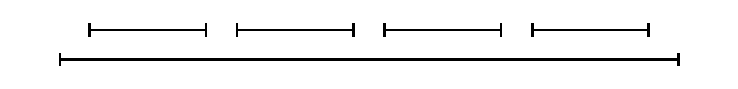
\includegraphics{fig70.pdf}
\end{center}
\end{frame}

\begin{frame}
 \frametitle{Eine zweite Idee}
 \begin{tabular}{p{0.5cm}p{10cm}} 
 (2) & Versucht man aus dem Fehlschlag der ersten Regel zu lernen, so könnte man auf die Idee kommen, \alert{immer ein möglichst kurzes Intervall} zu wählen -- dann können Effekte wie unter (1) nicht auftreten. Neue Regel: Man wähle immer diejenige Anfrage, für die $f(i)-s(i)$ so klein wie möglich ist.
\end{tabular}
\medskip

Diese Regel scheint etwas besser zu sein -- aber leider führt auch diese zu suboptimalen Ergebnissen, wie man am folgenden Beispiel erkennt:

\begin{center}
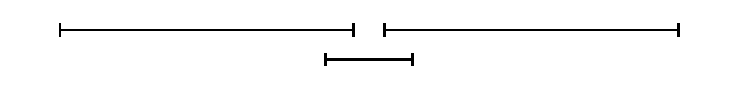
\includegraphics{fig71.pdf}
\end{center}

\end{frame}

\begin{frame}
\frametitle{Ein dritter Versuch}
 \begin{tabular}{p{0.5cm}p{10cm}} 
(3) & Bei der vorherigen Regel (2) lag das Problem darin, dass die zweite Anfrage sowohl mit der ersten als auch mit der dritten Anfrage inkompatibel war. Da ist es naheliegend, eine Regel aufzustellen, die besagt, dass \alert{immer eine Anfrage zu wählen ist, die mit möglichst wenigen anderen Anfragen kollidiert}. Das würde zumindest im Falle des Beispiels (2) helfen und scheint auch ansonsten recht vielversprechend zu sein: Man möchte ja insgesamt möglichst viele Anfragen akzeptieren; deshalb erscheint es einleuchtend, dass immer möglichst wenige Anfragen ausscheiden müssen.
\end{tabular}
\medskip

In der Tat muss man sich diesmal etwas mehr anstrengen, um ein entsprechendes Beispiel zu finden. Das folgende Beispiel zeigt jedoch, dass auch diese Regel suboptimale Ergebnisse liefert:

\begin{center}
 \includegraphics{fig72.pdf}
\end{center}
\end{frame}

\begin{frame}
 \frametitle{Und noch ein Versuch}
 \begin{tabular}{p{0.5cm}p{10cm}} 
 (4) & Nächster Versuch: Man richtet sich nach den Endzeiten der Anfragen und wählt immer diejenige Anfrage aus, für die $f(i)$ minimal ist. Auch für diese Regel gibt es ein Plausibilitätsargument: Je eher eine Anfrage beendet ist, desto eher kann die nächste Anfrage zum Zuge kommen.
\end{tabular}
\medskip

\alert{Nach unseren Erfahrungen mit den Regeln (1)--(3) sollten wir allerdings skeptisch sein:} Auch diesen Regeln lagen auf den ersten Blick einleuchtende Plausibilitätsargumente zugrunde. \\ \vspace*{0.2cm}

\alert{Allerdings fallen einem diesmal keine Beispiele ein, die die Suboptimalität der Regel (4) belegen}. So hat man den Verdacht, dass die vierte Regel (möglicherweise) immer eine optimale Lösung liefert. Um dies nachzuweisen, formulieren wir den dazugehörigen Algorithmus etwas formaler: Mit $R$ bezeichnen wir die \alert{Menge der Anfragen (engl. requests)}, über die noch zu entscheiden ist, die also bislang weder akzeptiert noch zurückgewiesen wurden; mit $A$ bezeichnen wir die \alert{Menge der bereits akzeptierten Anfragen}.
\end{frame}

\begin{frame}
 \frametitle{Intervall-Scheduling-Algorithmus}
 Hier nun der Algorithmus, den wir den \structure{Intervall-Scheduling-Algorithmus} nennen (nach Kleinberg/Tardos: \textit{Algorithm Design}):

\begin{center}
\begin{tabular}{rl}
\multicolumn{2}{l}{\textbf{Intervall-Scheduling-Algorithmus}} \\
& \\
 (1)& Am Anfang sei $R$ die Menge aller Anfragen und $A$ sei leer. \\
 (2)& \textbf{while} $R$ ist nicht leer. \\
 (3)& \qquad Wähle eine Anfrage $i \in R$ mit kleinster Endzeit. \\
 (4)& \qquad Füge $i$ zu $A$ hinzu. \\
 (5)& \qquad Lösche alle Anfragen in $R$, die nicht mit der Anfrage $i$ kompatibel sind. \\
 (6)& \textbf{end while} \\
 (7)& \textbf{return} die Menge $A$ als die Menge der akzeptierten Anfragen.
\end{tabular}
\end{center}

Im Skript finden Sie ein Beispiel, das den Ablauf des Intervall-Scheduling-Algorithmus illustriert (ebenfalls aus dem Buch von Kleinberg/Tardos).
\end{frame}

\begin{frame}
 \frametitle{Analyse}
 Im Folgenden befassen wir uns mit der \alert{Analyse des Intervall-Scheduling-Algorithmus}. Dabei geht es uns weniger um die Laufzeit, sondern vielmehr um die Korrektheit des Algorithmus: \\ \vspace*{0.2cm}
 
 Nachdem wir gesehen haben, dass das Greedy-Verfahren bei Verwendung der Regeln (1)--(3) nicht optimal arbeitet, wollen wir uns nun davon überzeugen, \alert{dass man bei Verwendung der Regel (4) \alert{immer} eine optimale Lösung erhält.}
\end{frame}

\begin{frame}
 \frametitle{$A$ und $\mathcal{O}$}
 In Zukunft wollen wir nicht mehr streng zwischen Anfragen und den dazugehörigen Intervallen unterscheiden. \\ \vspace*{0.2cm}
 
 Mit $A$ bezeichnen wir die Menge der Anfragen (Intervalle), die der Intervall-Scheduling-Algorithmus am Schluss liefert. Zum Zweck des Vergleichs betrachten wir außerdem eine optimale Lösung $\mathcal{O}$ des Problems. Wir haben zu zeigen, dass $A$ ebenfalls optimal ist, d.h.,\alert{ wir müssen
\[
|A| = |\mathcal{O}|
\]

zeigen.} \\ \vspace*{0.2cm}

Mit $i_1,\ldots,i_k$ wollen wir die Intervalle von $A$ bezeichnen -- in der Reihenfolge, in der sie vom Intervall-Scheduling-Algorithmus ausgewählt wurden. Dann gilt $f(i_r) \leq s(i_{r+1})$ für $r=1,\ldots,k-1$, d.h., die Intervalle von $A$ sind paarweise kompatibel und wie in der folgenden Zeichnung illustriert \enquote{von links nach rechts angeordnet}.
\end{frame}

\begin{frame}
\frametitle{$A$ und $\mathcal{O}$}
\begin{center}
\includegraphics{fig73.pdf}
\end{center}

Da $\mathcal{O}$ eine Lösung des Problems ist, überlappen sich auch die Intervalle von $\mathcal{O}$ nicht, d.h., die Intervalle von $\mathcal{O}$ liegen ebenfalls auf der reellen Achse \enquote{von links nach rechts angeordnet}. Dementsprechend wollen wir die Intervalle von $\mathcal{O}$ mit $j_1,\ldots,j_m$ bezeichnen, wobei $f(j_r) \leq s(j_{r+1})$ für alle $r=1,\ldots,m-1$ gilt. \\ \vspace*{0.2cm}

Da $\mathcal{O}$ eine optimale Lösung ist, gilt $k \geq m$; unser Ziel ist es, $k=m$ nachzuweisen. \alert{Um dies zu erreichen, zeigen wir (Dies ist der entscheidende Schritt!), dass Folgendes gilt:
\begin{equation}
\label{eq:12:1}
f(i_r) \leq f(j_r) \quad \text{für alle } r = 1,\ldots,k.
\end{equation}}
\end{frame}

\begin{frame}
 \frametitle{Der Intervall-Scheduling-Algorithmus liegt immer vorn!}
 Dasselbe in Worten: \alert{Für alle Intervalle $i_r$ von $A$ vergleichen wir den rechten Randpunkt $f(i_r)$ mit dem rechten Randpunkt $f(j_r)$ des entsprechende Intervalls $j_r$ von $\mathcal{O}$ und behaupten, dass $f(i_r)$ niemals rechts von $f(j_r)$ liegt}. Dies ist der präzise Inhalt der Feststellung, dass unser Intervall-Scheduling-Algorithmus \enquote{immer vorne liegt}. \\ \vspace*{0.2cm}

 Den Beweis von \eqref{eq:12:1} betrachten wir nicht, dieser kann im Skript gefunden werden. 
\end{frame}

\begin{frame}
 \frametitle{Nachweis von $k=m$}
 Nachdem \eqref{eq:12:1} als richtig erkannt wurde, fällt der Nachweis von $k=m$ nicht schwer: \\ \vspace*{0.2cm}
 
 \alert{Angenommen es gelte $k<m$.} Dann gibt es ein Intervall $j_{k+1}$ in $\mathcal{O}$ und es gilt $f(j_k) \leq s(j_{k+1})$. Wegen \eqref{eq:12:1} gilt außerdem $f(i_k) \leq f(j_k)$. Es folgt $f(i_k) \leq s(j_{k+1})$. Dies würde jedoch Folgendes bedeuten: Nachdem am Ende unseres Intervall-Scheduling-Algorithmus $i_k$ ausgewählt wurde, \alert{ist immer noch das Intervall $j_{k+1}$ in $R$.} Dieser Widerspruch beweist $k=m$.
\end{frame}

\begin{frame}
 \frametitle{Nun: Austauschargument}
 Wir haben somit ein Beispiel für die Methode

\begin{center}
\alert{The Greedy Algorithm Stays Ahead}
\end{center}

kennengelernt. Im Buch von Kleinberg und Tardos finden sich noch viele interessante Ergänzungen sowohl zu dieser Methode als auch zum Thema Intervall-Scheduling. Wir fahren nun fort mit der zweiten Methode, die den Namen

\begin{center}
\alert{Austauschargument}
\end{center}

trägt.
\end{frame}

\begin{frame}
 \frametitle{Ein weiteres Scheduling-Problem} 
Es geht auch hier wieder um ein Schedulingproblem -- diesmal sollen jedoch \alert{alle} Anfragen akzeptiert werden, wobei es allerdings zu \alert{Verspätungen} kommen kann. \\ \vspace*{0.2cm}

\textbf{Genauer:} Wir haben wieder eine Ressource, die wir uns als eine \alert{Maschine} vorstellen wollen, an der immer nur ein \alert{Job} zur selben Zeit erledigt werden kann; statt \enquote{Anfrage} wollen jetzt immer \enquote{Job} sagen. Es gebe $n$ Jobs und jeder Job besitze eine \alert{Ausführungszeit} $t_i > 0$; Anfangs- und Endpunkt eines Jobs sollen diesmal aber nicht feststehen -- stattdessen soll es eine \alert{Deadline} $d_i$ für jeden Job geben.
\end{frame}

\begin{frame}
 \frametitle{Ein weiteres Scheduling-Problem}
 Wir nehmen an, dass die Maschine zum Zeitpunkt $s$ bereitsteht. Die Jobs seien mit $1,\ldots,n$ bezeichnet. Jedem Job $i$ ist ein Intervall $[s(i), f(i)]$ zuzuordnen, wobei gelten soll:
\[
s \leq s(i) \quad \text{und} \quad f(i)-s(i) = t_i \quad (i=1,\ldots,n).
\]

\textbf{Klar ist:} Die Intervalle $[s(i),f(i)]$ sollen sich nicht überlappen. \\ \vspace*{0.2cm}
\textbf{Was ist nun aber zu optimieren?} Es gibt verschiedene Möglichkeiten, die zu Problemen von unterschiedlichem Schwierigkeitsgrad führen. Wir wollen hier die \alert{Variante} betrachten, \alert{bei der die maximale Verspätung zu minimieren ist}.
\end{frame}

\begin{frame}
 \frametitle{Die maximale Verspätung}
 Wir nennen den Job $i$ \structure{verspätet}, falls $d_i < f(i)$ gilt; wir setzen
\[
\ell_i = 
\begin{cases}
f(i) - d_i & \text{, falls der Job  $i$ verspätet ist}; \\
0 & \text{, falls der Job $i$ nicht verspätet ist}.
\end{cases}
\]
Man nennt $\ell_i$ die \structure{Verspätung} des $i$-ten Jobs. \\ \vspace*{0.2cm}

Zu minimieren ist
\[
L = \max{\big\{ \ell_i : i = 1,\ldots,n \big\}}.
\]
Wie könnte ein Greedy-Algorithmus für unser Problem aussehen? \\ \vspace*{0.2cm}

Es bieten sich wieder etliche Möglichkeiten an, den Jobs\index{Job} mithilfe einer einfachen Regel Zeitintervalle zuzuordnen:
\end{frame}

\begin{frame}
\frametitle{Ein erster Versuch}
\begin{tabular}{p{0.5cm}p{10cm}} 
(1) & Eine dieser Möglichkeiten wäre, \alert{die Jobs zunächst nach aufsteigender Länge $t_i$ zu ordnen und ihnen dann in dieser Reihenfolge nach dem Motto \enquote{die Kleinen zuerst} ein Zeitintervall zuzuordnen}; zumindest im obigen Beispiel hat das geklappt -- die kleinen Jobs so früh wie möglich aus dem Weg zu kriegen, könnte eine gute Idee sein.
\end{tabular}
\medskip

Andererseits werden bei dieser Strategie die Deadlines überhaupt nicht berücksichtigt; man braucht sich also nicht zu wundern, dass es \enquote{schlechte Beispiele} bereits dann gibt, wenn nur zwei Jobs im Spiel sind:

\begin{center}
\begin{tabular}{rl}
1. Job: & $t_1=1,\quad d_1=100$; \\
2. Job: & $t_2=10, \quad d_2=10$.
\end{tabular}
\end{center}
\end{frame}

\begin{frame}
\frametitle{Zweiter Versuch}
\begin{tabular}{p{0.5cm}p{10cm}} 
(2) & Das Beispiel zu (1) legt nahe, mehr auf die \enquote{slack time} $d_i - t_i$ zu achten und \alert{die Jobs vorzuziehen, für die $d_i-t_i$ klein ist:} Diese Jobs vertragen nur wenig Aufschub und sollten deshalb so schnell wie möglich erledigt werden.
\end{tabular}
\medskip

Leider verfehlt auch diese Greedy-Regel ihr Ziel; man betrachte das folgende Beispiel:

\begin{center}
\begin{tabular}{rl}
1. Job: & $t_1=1, \quad d_1=2$; \\
2. Job: & $t_2=10, \quad d_2=10$.
\end{tabular}
\end{center}
\end{frame}

\begin{frame}
 \frametitle{Earliest Deadline First}
 \begin{tabular}{p{0.5cm}p{10cm}} 
(3) & Nun kommt eine Regel, die genauso einfach wie die beiden anderen ist, von der sich aber herausstellen wird, dass sie immer eine optimale Lösung liefert: \alert{Man ordnet die Jobs nach ihren Deadlines, wobei die frühen Deadlines zuerst drankommen;} diese Regel ist unter dem folgenden Namen bekannt:
\begin{center}
\alert{Earliest Deadline First}
\end{center}
\end{tabular}
\medskip

So einfach geht das? Und das soll funktionieren? \alert{Man hat allen Grund gegenüber dieser Regel skeptisch zu sein:} Beispielsweise war einer der Einwände gegen die Regel (1), dass sie die Hälfte der Eingangsdaten -- die Deadlines $d_i$ -- gar nicht berücksichtigt. \alert{Und nun soll eine Regel optimal sein, die die andere Hälfte der Eingangsdaten -- die Intervalllängen $t_i$ -- komplett ignoriert?}
\end{frame}

\begin{frame}
 \frametitle{Ein Plausibilitätsargument}
 Es gibt natürlich \alert{Plausibilitätsargumente} für die Regel (3): Beispielsweise könnte man argumentieren, dass ein Job, der früh erledigt sein muss, auch früh angefangen werden sollte. Andererseits: Was von solchen Plausibilitätsargumenten zu halten ist, haben wir ja bereits gesehen. \\ \vspace*{0.2cm}

Es soll nun \alert{nachgewiesen} werden, dass die Regel \alert{Earliest Deadline First} immer eine optimale Lösung hervorbringt. \\ \vspace*{0.2cm}

Wir starten damit, dass wir die Jobs neu benennen: Die Bezeichnungen $1,\ldots,n$ für die Jobs sollen in der Reihenfolge der Deadlines vergeben werden, d.h., es soll
\[
d_1 \leq \ldots \leq d_n
\]

gelten. Unsere Strategie besagt dann, dass
\begin{itemize}
\item Job 1 die Startzeit $s(1)=s$ und die Endzeit $f(1)=s(1)+t_1$ erhält;
\item Job 2 die Startzeit $s(2) = f(1)$ und die Endzeit $f(2) = s(2) + t_2$ bekommt;
\item usw. 
\end{itemize}
Als erstes beobachten wir, dass dieser Algorithmus einen Zeitplan (engl. schedule) liefert, bei dem es \alert{keine Lücken} gibt.
\end{frame}

\begin{frame}
 \frametitle{Nochmals $A$ und $\mathcal{O}$}
 Ferner ist klar, dass es auch einen optimalen Zeitplan ohne Lücken gibt, da Lücken leicht beseitigt werden können, ohne die Optimalität zu zerstören. Optimal bedeutet in unserem Fall natürlich immer, dass 
 $$L=\max{\bigl\{ \ell_i : i = 1,\ldots,n \bigr\}}$$
 so klein wie möglich ist. \\ \vspace*{0.2cm}

Wir nennen den von unserem Greedy-Algorithmus produzierten Zeitplan $A$; mit $\mathcal{O}$ sei ein optimaler Zeitplan bezeichnet.
\end{frame}

\begin{frame}
 \frametitle{Austauschargument}
Unser Ziel ist, $\mathcal{O}$ durch schrittweise Änderung in $A$ zu überführen, wobei \alert{in jedem Änderungsschritt die Optimalität erhalten bleiben soll.} Diese Vorgehensweise nennen wir \structure{Austauschargument}. \\ \vspace*{0.2cm}

Wir sagen, dass in einem gegebenen Zeitplan eine \structure{Inversion} vorkommt, falls es in diesem Zeitplan zwei Jobs $i$ und $j$ gibt, für die gilt: $i$ liegt in diesem Zeitplan vor $j$, obwohl $d_j < d_i$ gilt.
\end{frame}

\begin{frame}
 \frametitle{Zeitplänne ohne Inversionen und Lücken}
 Man beachte, dass unser Zeitplan $A$ keine Inversionen besitzt. Falls es verschiedene Jobs mit gleicher Deadline gibt, so könnte es außerdem etliche andere Zeitpläne ohne Inversionen und ohne Lücken geben. Wir zeigen nun, dass alle diese Zeitpläne dieselbe maximale Verspätung $L$ besitzen.

\begin{align}
\label{eq:12:*}
\tag{$\star$}
\begin{split}
&\alert{\text{Alle Zeitpläne ohne Inversionen und ohne Lücken}} \\
&\alert{\text{besitzen dieselbe maximale Verspätung.}}
\end{split}
\end{align}

\textbf{Beweis:} Falls zwei verschiedene Zeitpläne weder Inversionen noch Lücken besitzen, dann können sie sich nur dadurch unterscheiden, dass Jobs mit gleicher Deadline in unterschiedlicher Reihenfolge ausgeführt werden. Es sei $d$ eine solche Deadline. In beiden Zeitplänen liegen die Jobs mit Deadline $d$ dann lückenlos aneinandergereiht -- nur eben in unterschiedlicher Reihenfolge. Unter diesen Jobs mit Deadline $d$ besitzt der letzte die größte Verspätung -- und diese ist unabhängig von der Reihenfolge dieser Jobs. \qquad $\Box$
\end{frame}

\begin{frame}
 \frametitle{Wie funktioniert das Austauschargument}
 \textbf{Wie funktioniert nun das Austauschargument?} Wir schildern hier nur die \alert{Grundidee}; die Details findet man im Buch von Kleinberg/Tardos. \\ \vspace*{0.2cm}
 
 Man startet von einem optimalen Zeitplan $\mathcal{O}$ ohne Lücken; dass es einen solchen Zeitplan gibt, haben wir bereits festgestellt. $\mathcal{O}$ wird nun schrittweise abgeändert, \alert{wobei in jedem Schritt ein Paar von benachbarten Intervallen die Reihenfolge wechselt und alle anderen Intervalle unverändert bleiben}. 
\end{frame}

\begin{frame}
 \frametitle{Wie funktioniert das Austauschargument?}
 Dies geschieht so, dass gilt:
\begin{itemize}
\item Die auftretenden Zeitpläne haben niemals Lücken.
\item In jedem Schritt sinkt die Anzahl der Inversionen um 1.
\item In keinem Schritt vergrößert sich $L$, d.h., alle auftretenden Zeitpläne bleiben optimal.
\end{itemize}

Nach endlich vielen Schritten erhält man somit einen optimalen Zeitplan, der keine Inversionen und keine Lücken aufweist. \\ \vspace*{0.2cm}

Damit ist gezeigt, dass ein optimaler Zeitplan ohne Inversionen und ohne Lücken existiert. \alert{Da unser Zeitplan $A$ ebenfalls weder Lücken noch Inversionen aufweist, folgt wegen \eqref{eq:12:*}, dass auch $A$ optimal ist.}
\end{frame}

\end{document}
